The human genome is the complete set of nucleic acid sequences for humans, encoded as DNA (deoxyribonucleic acid) within the 23 chromosome pairs, adding up to 6.4 billion base pairs \cite{WIKI:HumanGenome}. The DNA is divided in sequences called \textit{gene}, the basic unit of heredity. Every person has two copies of each gene, one inherited from each parent. Most genes are the same in all people, but a small number of genes (less than 1 percent of the total) are slightly different between people. These small differences contribute to each person's unique physical features. In humans, genes vary in size from a few hundred DNA bases to more than 2 million bases \cite{Gene}. A \textit{base} (nucleotide) is the fundamental unit which codifies the DNA (adenine (A), cytosine (C), guanine (G) and thymine (T)) and RNA (like DNA but uracil (U) instead of thymine).\newline
In this thesis is discussed the implementation of a NGS (Next Generation Sequencing) pipeline, which aims to detect \textbf{variants} (mutations) of a human genome from a reference genome. These variants are then loaded in databases and statistical tools, in order to identify harmful mutations. Variants called inside this pipeline include SNPs (Single Nucleotide Polymorphism) and INDELs (insertions/deletions).\newline
\textbf{SNP} is the most common type of genetic variation among people and represents a difference of a DNA nucleotide (for example, a SNP may replace the nucleotide cytosine (C) with the nucleotide thymine (T) in a certain point of DNA). They can act as biological markers, to locate genes that are associated with disease. SNPs can also be used to track the inheritance of disease genes within families. Future studies will work to identify SNPs associated with complex diseases such as heart disease, diabetes, and cancer \cite{SNP}.\newline
An \textbf{INDEL} polymorphism is a variation in which a specific nucleotide sequence is present (insertion) or absent (deletion). While not as common as SNPs, INDELs are widely spread across the genome \cite{INDEL}.
\begin{figure}[h] 
\begin{center}
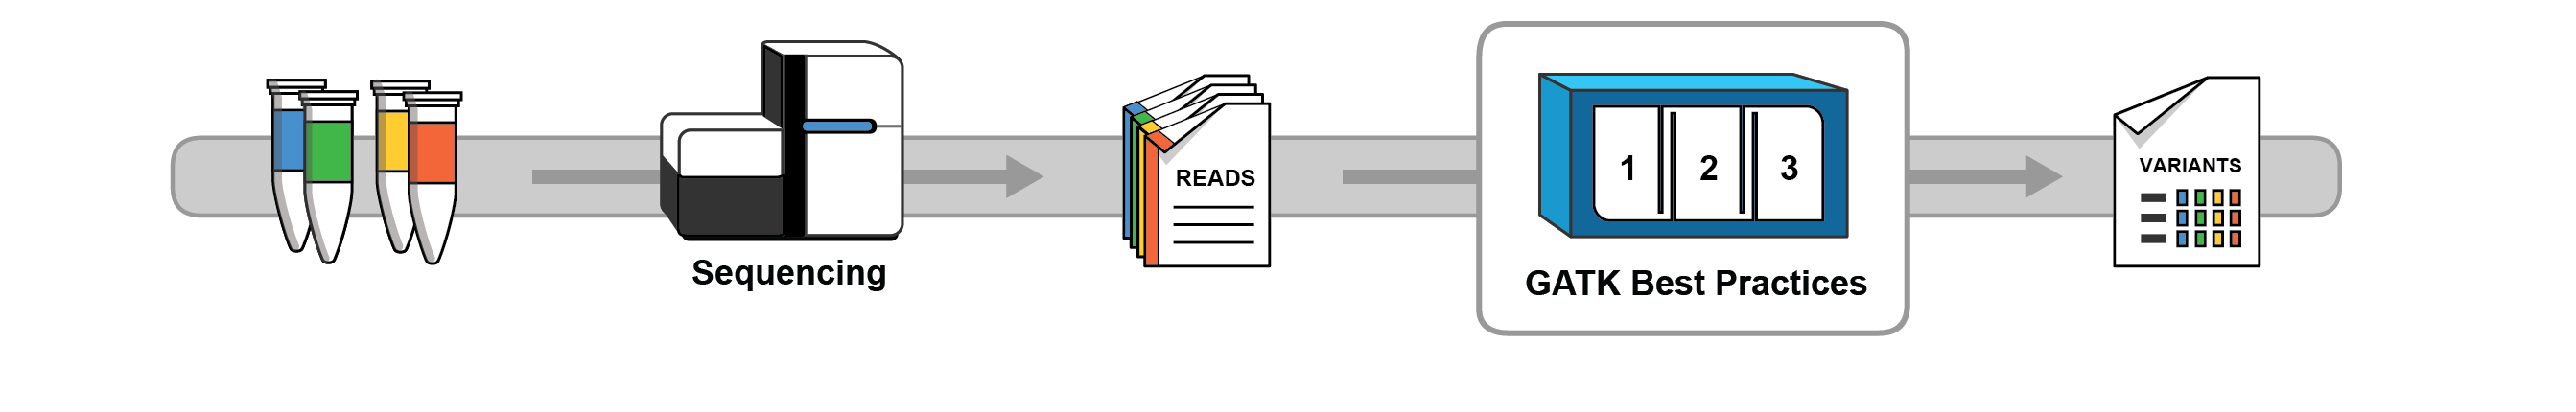
\includegraphics[scale=0.51]{figure/pipeline_overview.png}
\end{center}
\caption{Pipeline Overview ~\label{pipeline_overview}}
\end{figure}
\\[1\baselineskip]
As shown in Figure ~\ref{pipeline_overview}, this human genome processing starts with a biological sample (e.g. blood, saliva...) as input of sequencing machines and finishes with a report of differences from the reference genome and what they mean. This is usually divided into three stages:
\begin{enumerate}
	\item Primary analysis: analyses a sample
biochemically and produces raw data
	\item Secondary analysis: takes the raw data,
aligns it to the reference, and identifies variants
(differences) from the reference
    \item Tertiary analysis: analyses the variants
and adds annotations to help interpret their
biological or clinical implications
\end{enumerate}
The primary analysis stage is done in the laboratory using specialized \textbf{sequencing} instruments. The genome sequencer replicates and fragments the DNA and then reads the base pairs, in a massively parallel process combining biochemistry, optics, electronics, and image processing. Identifying the base pairs in a sequence of DNA (base calling) is hard and errors do happen, so in addition to the A, C, T, or G base called for each location, the sequencer also produces a \textit{quality score} to record how confident the sequencer is in the base call. Sequencing an entire human genome typically produces about a billion roughly 100-250 character strings (\textbf{reads}) of A, C, T, and G (bases), covering the genome with an average of 30 copies for redundancy, over-sampling the DNA.\newline
Ideally, DNA sequencing includes the entire genome, Whole-Genome Sequencing (WGS).
While WGS technology is rapidly coming on the market at affordable prices, in the last few years most research labs have adopted \textbf{Whole-Exome Sequencing} (WES) as interim technology. WES is limited to the exome information, that is to the regions of DNA that are responsible for protein expression by way of RNA translation. These are the priority areas of the genome, where mutations can be more easily identified as deleterious, as they have a higher chance of directly compromising protein synthesis. WES-based diagnosis provides a good trade-off between diagnostic power and the cost of data processing, as exomes only account for about 1.5\% of the entire genome and can, therefore, be processed using in-house computational resources \cite{ScalableEfficientWhole-ExomeProcessing}.\newline
This process produces about 15 GB of compressed WES raw data per sample (instead of 1 TB for WGS) ready for secondary analysis, typically stored in FASTQ files. In particular we talk about \textit{paired end reads}, which means that a DNA fragment is sequenced in both ends, generating high quality sequence data collected in 2 FASTQ files \cite{PairedEnd, MicrosoftGenomics}.
\\[1\baselineskip]
This project focuses on second and third stage, the process that goes from \textit{reads} to \textit{variants} discovery and annotation illustrated in ~\ref{pipeline_overview} and deepened in next paragraphs.
\section{GATK Best Practices}
The FASTQ files produced from the sequencing machine are used as input of the GATK tools: here begins the Big Data processing. Indeed these tools take over a day to process a 30x whole genome sample on a 16-core server, starting with the FASTQ files from the sequencer, and producing a file of aligned reads and a file of variant calls.\newline
In a discovery approach, I used the GATK tutorials in order to follow their Best Practices, which can be divided in 3 phases (as even the Best Practices Figure~\ref{best_practices} are divided): Preprocessing, Variant Discovery and Call Set Refinement; at the time was available GATK version 3.8 and it was possible to execute their tools step by step. The basic concept of this pipeline is that each tool processes the file generated by the previous tool, in a sequential manner.
\begin{figure}[h] 
\begin{center}
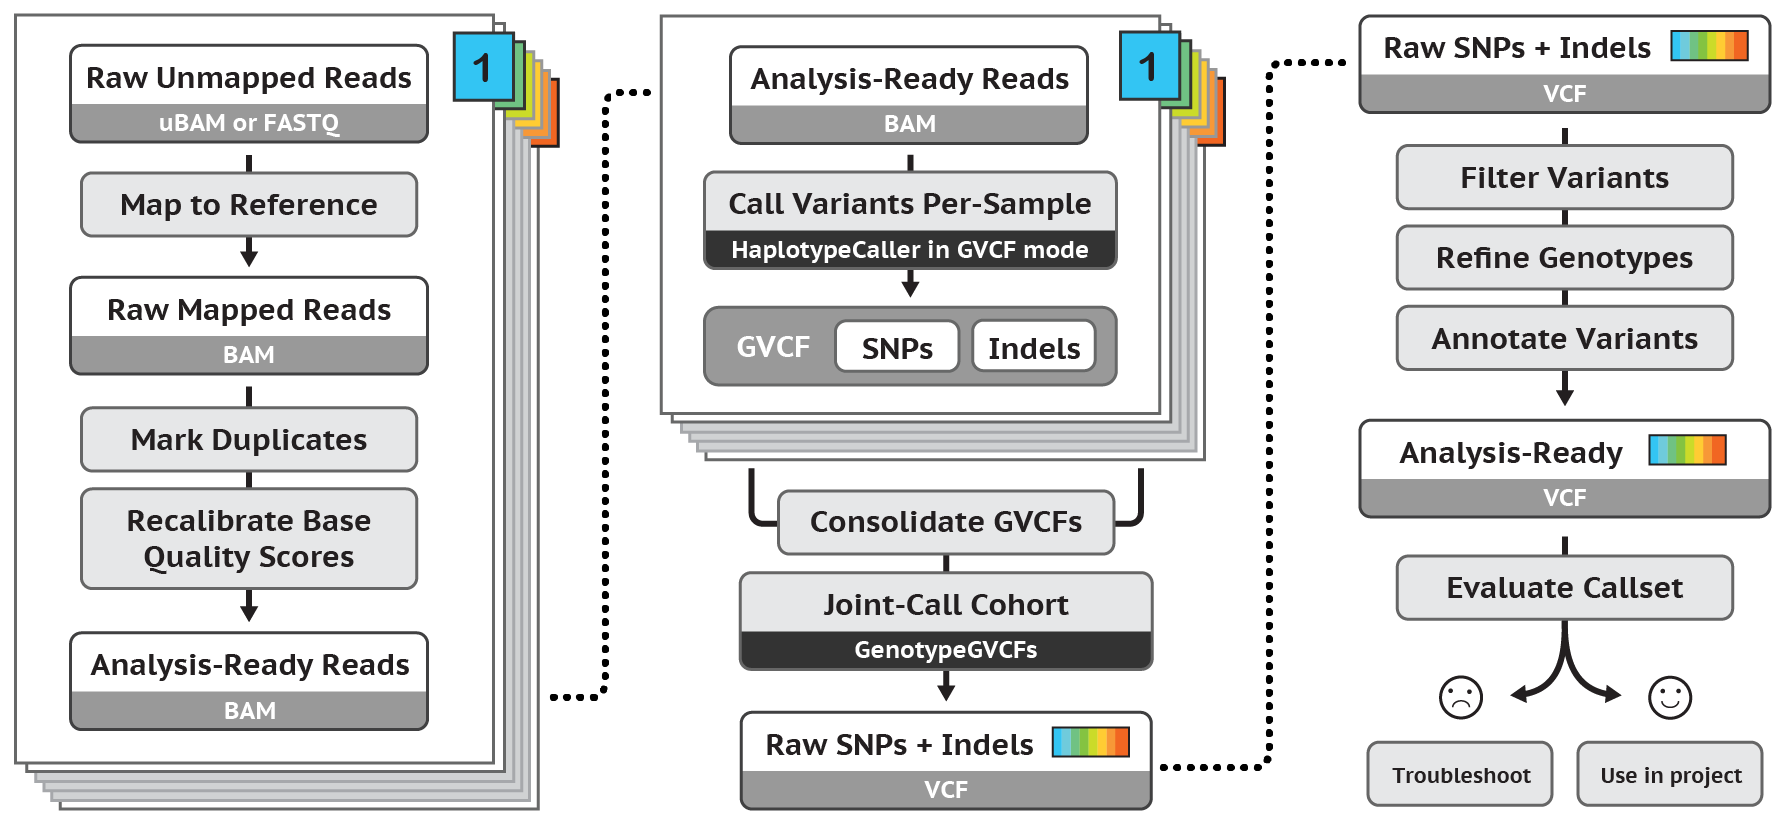
\includegraphics[scale=0.31]{figure/best_practices.png}
\end{center}
\caption{GATK Best Practices ~\label{best_practices}}
\end{figure}
\subsection{Preprocessing}
The Preprocessing phase is the most resource and time consuming phase. As is possible to observe in the Best Practices Figure ~\ref{best_practices}, this phase goes from the \textit{Raw Unmapped Reads} to the \textit{Recalibrate Base Quality Score} (but I included here even HaplotypeCaller in GVCF mode, because of designing decision), and the tools used here must process each of the human genomes in input (the FASTQ files) in a sequential manner.
\\[1\baselineskip]
Since human DNA varies relatively little among individuals (typically about 1 in 1000 locations) we usually compare a given person's DNA to a reference genome, a composite genome based on the results of the first Human Genome Project \cite{MicrosoftGenomics}. So this is the first step, aligning the sequenced reads collected in FASTQ files against a human reference genome, mapping each read to one or more positions, in order to reconstruct the sequenced genome. For this pipeline was used the reference genome HG19, but the only reference file is not enough: are necessary even indexes of the reference genome, for which GATK provides tools that allow to create them. Indexes are necessary to other tools in order to improve access performance to reference genome. A \textit{de facto standard} software for the alignment is the \textbf{Burrows Wheeler Aligner}, in particular using the algorithm \textbf{BWA-MEM} \cite{BWA}. The output generated by this software is stored in a SAM (Sequence Alignment Map) file. \newline
After that, using tools provided by Picard, the reads inside the SAM file will be \textbf{sorted}, for then \textbf{Marking Duplicates}: a process that flags the paired reads mapped to exactly the same start and end positions as duplicates. These reads often originate erroneously from DNA preparation methods. They will cause biases that skew variant calling and hence should be removed, in order to avoid them in downstream analysis; this process generates a BAM (Binary Alignment Map, a compressed binary representation of SAM) file \cite{Picard}. \newline
The following step is the \textbf{BQSR} (Base Quality Score Recalibration): since that the sequencing machine emits error (for example due to physics or chemistry of how the sequencing reaction works), for each base call is even provided a quality score, which represents how confident the machine was that it called the correct base. Here a machine learning approach adjusts these scores \cite{BQSR}. Known sites (which will be discussed in Datasets chapter) are required in order to execute this step.\newline
Even if \textbf{Haplotype Caller} is considered part of Variant Discovery phase, I treated here because of designing reasons. Indeed it aims to call variants on a single genome, to discovery germline variants in DNA. But as previous tools, this must process each of the DNA sample (in particular the output file generated by the previous tool). The output file is a raw (unfiltered) VCF (Variant Calling Format). This tool calls SNPs and INDELs simultaneously.

\subsection{Variant Discovery}
After that all the previous steps processed each human genome sample in input (in other words, the Haplotype Caller generated a raw VCF file for each human genome), it is possible to execute the \textbf{GenotypeGVCFs}. As possible to notice in the Best Practices Figure ~\ref{best_practices}, this tool takes in input the VCF files generated from Haplotype Caller (in particular, since the GATK version 3, the file extension of Haplotype Caller is .g.vcf) to create the raw SNP and INDEL VCF that are usually emitted by the callers \cite{HaplotypeCaller}. From this point of the pipeline the execution goes on with a single file: the file produced from a tool will be the input for the following tool.\newline
Following this approach, is now necessary to apply \textbf{VQSR} (Variant Quality Score Recalibration), a method that uses machine learning algorithms to learn from each dataset what is the annotation profile of good variants vs. bad variants, and does so in a way that integrates information from multiple dimensions (5 to 8 typically). This allows us to pick out clusters of variants in a way that frees us from the traditional binary choice of "is this variant above or below the threshold for this annotation?" \cite{VQSR1,VQSR2}. This is possible through the \textbf{Variant Recalibrator} and \textbf{Apply Recalibration} tools, in order to recalibrate variant quality scores and produce a callset filtered for the desired levels of sensitivity and specificity. In particular the process is so structured:

\begin{enumerate}
	\item Prepare recalibration parameters for SNPs
	\begin{enumerate}
    	\item Specify which call sets the program should use as resources to build the recalibration model
    	\item Specify which annotations the program should use to evaluate the likelihood of INDELs being real
    	\item Specify the desired truth sensitivity threshold values that the program should use to generate tranches
    	\item Determine additional model parameters
    \end{enumerate}

	\item Build the SNP recalibration model
	\item Apply the desired level of recalibration to the SNPs in the call set
	\item Prepare recalibration parameters for INDELs 
    	\begin{enumerate}
    	\item Specify which call sets the program should use as resources to build the recalibration model 
    	\item Specify which annotations the program should use to evaluate the likelihood of INDELs being real 
    	\item Specify the desired truth sensitivity threshold values that the program should use to generate tranches 
    	\item Determine additional model parameters
    \end{enumerate}
	\item Build the INDEL recalibration model
	\item Apply the desired level of recalibration to the INDELs in the call set
\end{enumerate}
At the end of this process, a file containing the recalibrated variants is produced \cite{runVQSR}.

\subsection{Call Set Refinement}
This phase of the pipeline, according to GATK Best Practices \ref{best_practices}, starts with the \textbf{Genotype Refinement}; it takes in input the VCF file generated by the previous VQSR and it is composed of three steps:
\begin{enumerate}
\item Derive posterior probabilities of genotypes: we are deriving the posteriors of genotype calls in our callset, the VCF file generated by VQSR.
\item Filter low quality genotypes: after the posterior probabilities are calculated for each sample at each variant site, genotypes with GQ < 20 based on the posteriors are filtered out. GQ20 is widely accepted as a good threshold for genotype accuracy, indicating that there is a 99\% chance that the genotype in question is correct. Tagging those low quality genotypes indicates to researchers that these genotypes may not be suitable for downstream analysis (a filter tag is applied, but the data is not removed from the VCF).
\item Annotate possible de novo mutations: using the posterior genotype probabilities, possible de novo mutations are tagged \cite{GenotypeRefinement}.
\end{enumerate}
Finally there is the \textbf{Variant Annotation} process, which is not supported by GATK. Indeed their tutorial suggests to use third-party software. There is a wide variety of tools and databases in use for this process. Depending on the purpose of the analysis, these might add information about evolutionary conservation, protein structure, drug response, disease risk, genomic interactions, etc. The choice of databases and tools depends greatly on the purpose of the analysis, and the overall methodology of the clinician or researcher.\newline
Due to union of VCF files in only one through GenotypeVCFs, the current VCF file at this point of the pipeline is a sort of a CSV file with many fields, among which the input samples names. But now is necessary to split this VCF in many file as the number of input samples, since that following annotation steps require a VCF relative to each sample. In order to deliver this task, GATK provides the tool \textit{SelectVariants}, which allows us to do it. From this point of the pipeline to the end, we have the same approach used during the Preprocessing phase, where each tool processed each sample; here each tool annotates each sample.
\\[1\baselineskip]
As a first annotation tool here we used \textbf{ANNOVAR}, an efficient software tool (a command line Perl program) that allows to functionally annotate genetic variants detected from diverse genomes. This is possible through well known Databases in literature, that ANNOVAR allows to download. It is used extensively by the scientific community. This efficient program enables annotation of a whole genome in less than four minutes and filtering of important variants in less than 15 minutes \cite{ANNOVAR}.
Finally the pipeline concludes with the annotation though \textbf{IGM Anno} and a filtering called \textbf{Exonic Filter}. The finally VCF file generated in this last step were comparable with the VCF realized in another pipeline.

\section{Hadoop Distributed File System (HDFS)}
The Hadoop Distributed File System (HDFS) is a distributed file system designed to run on commodity hardware (scale "out" rather than "up" ), designed to be highly fault-tolerant and deployed on low-cost hardware. HDFS provides high throughput access to application data and is suitable for applications that have large data sets.
\begin{figure}[h] 
\begin{center}
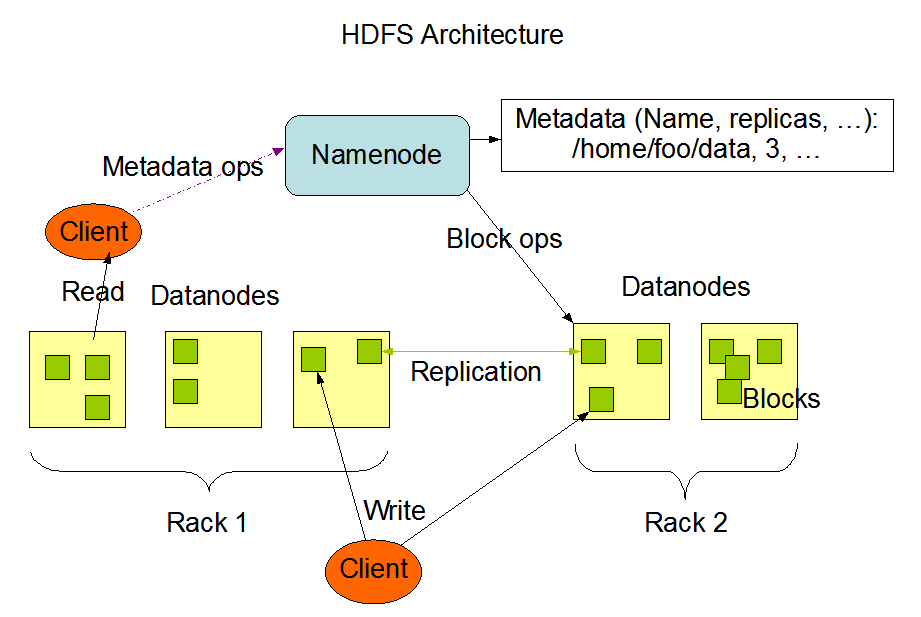
\includegraphics[scale=0.4]{figure/HadoopArch.png}
\end{center}
\caption{HDFS Architecture ~\label{services_swarm}}
\end{figure}
\\[1\baselineskip]
HDFS has a master/slave architecture. An HDFS cluster consists of a single \textbf{NameNode}, a master server that manages the file system namespace and regulates access to files by clients. In addition, there are a number of \textbf{DataNodes}, usually one per node in the cluster, which manage storage attached to the nodes that they run on. HDFS exposes a file system namespace and allows user data to be stored in files. Internally, a file is split into one or more blocks and these blocks are stored in a set of DataNodes. The NameNode executes file system namespace operations like opening, closing, and renaming files and directories. It also determines the mapping of blocks to DataNodes. The DataNodes are responsible for serving read and write requests from the file system's clients \cite{HDFS}.
\\[1\baselineskip]
In this project HDFS has been necessary in order to distribute mandatory files for the pipeline over the cluster. Some GATK tools in cluster mode expect to find in input HDFS files path.

\section{Apache Spark}
Since that NGS pipelines process big quantity of data, Apache Spark is a fast and general-purpose cluster computing system. It would introduce efficiency in these pipelines not only because allows to distribute the work load on a cluster of more computers, but even because runs programs up to 100x faster than \textit{Hadoop MapReduce}. This is due to Spark in-memory data storage, for very fast iterative queries, using general execution graphs and powerful optimizations. Provides high-level APIs in Java, Scala, Python and R, and can run on top of Hadoop Cluster.

\subsection{Cluster Architecture}
Spark applications run as independent sets of processes on a cluster, coordinated by the \textbf{SparkContext} object in the main program (\textbf{Driver Program} which is situated in \textit{Driver node}), according to the developer requirements. There is another machine where the Spark cluster manager is running, called the \textit{Master node}. Along side, in each of the machines in the cluster, there is a \textit{Worker} process running which reports the available resources in its node to the \textit{Master}. Once connected, Spark acquires \textbf{Executors} on nodes in the cluster (\textit{Worker nodes}), which are processes that run computations and store data for the application. After that it sends the application code (defined by high-level APIs) to the executors. Finally, SparkContext sends tasks to the executors to run. \newline
In other words, when the \textit{Driver} process needs resources to run jobs/tasks, it ask the \textit{Master} for some resources. The \textit{Master} allocates the resources and uses the \textit{Workers} running through out the cluster to create \textit{Executors} for the \textit{Driver}. Then the Driver can run tasks in those \textit{Executors}.\newline
\begin{figure}[h] 
\begin{center}
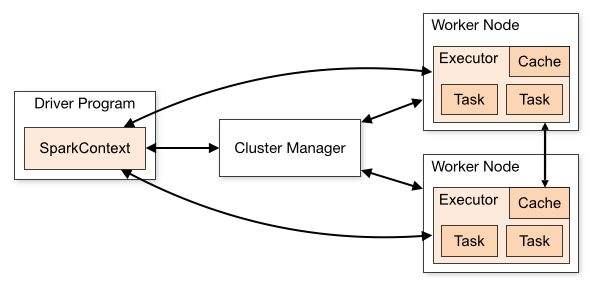
\includegraphics[scale=0.66]{figure/spark-cluster-overview.png}
\end{center}
\caption{Apache Spark Cluster overview~\label{spark_cluster}}
\end{figure}
Each application gets its own executor processes, which stay up for the duration of the whole application and run tasks in multiple threads. This has the benefit of isolating applications from each other, on both the scheduling side (each driver schedules its own tasks) and executor side (tasks from different applications run in different JVMs).\newline
Spark revolves around the concept of \textbf{Resilient Distributed Dataset} (RDD), distributed collections of objects that can be cached in memory
across cluster nodes. It is fault-tolerant (automatically rebuilt on failure) and can be operated on in parallel. RDD are the distributed memory abstractions that lets programmer perform in-memory parallel computations on large clusters in a highly fault tolerant manner.\newline
When the user application creates RDDs and run actions, the result is a DAG (Directed Acyclic Graph) of operators, which is compiled into stages. Each stage is executed as a series of Task (one Task for each Partition) \cite{Spark}.
\\[1\baselineskip]
Even GATK in the 4th version introduced Spark because of all these benefits. So in this moment some of their tools support Spark; for other tools which are not in Spark, I implemented them in a manner discussed in next chapters, in order to introduce Spark in them too.

\section{Docker}
Docker is a platform to develop, deploy, and run applications with containers. The use of Linux containers to deploy applications is called containerization. Containerization is increasingly popular because containers are: \textit{lightweight} (containers leverage and share the host kernel), \textit{interchangeable} (deploy updates and upgrades on-the-fly), \textit{portable} (build locally, deploy to the cloud, and run anywhere) and \textit{scalable} (possibility to increase and automatically distribute container replicas).\newline
A container is launched by running an \textbf{image}, an executable package that includes everything needed to run an application (the code, a runtime, libraries, environment variables, and configuration files). So a container is a runtime instance of an image (what the image becomes in memory when executed).\newline
The Figure ~\ref{container_vm} shows the difference between Docker Container and a generic Virtual Machine: containers are used to execute one or more specific applications, defining a virtual environment required by an application set. Host does not need an hypervisor. Containers do not have the complete OS (the only constraint is a compatible host OS), contain only the strictly necessary to execute an application and decoupling it from the underlying system. Containerized software will always run the same, regardless of the environment.
\begin{figure}[h] 
\begin{center}
\begin{tabular}{c @{\hspace{1em}} c}
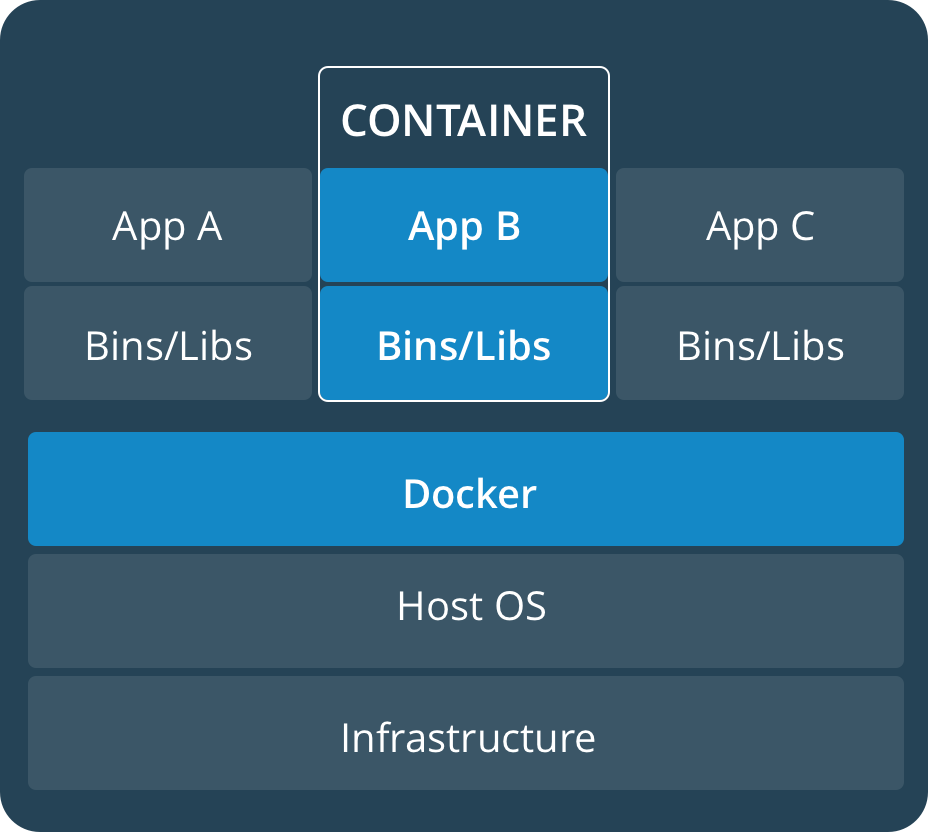
\includegraphics[scale=0.225]{figure/Container.png} &
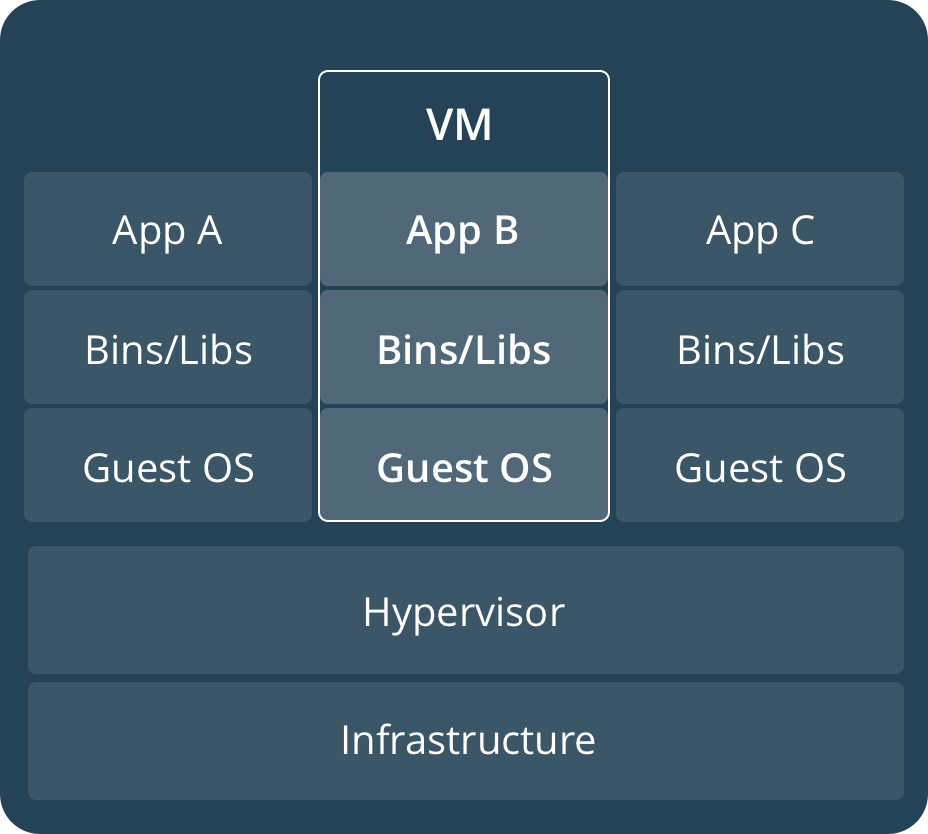
\includegraphics[scale=0.225]{figure/VM.png} \\
 (a - Docker Container) & (b - Virtual Machine)
\end{tabular}
\end{center}
\caption{Comparison of Docker Container and Virtual Machine. ~\label{container_vm} \newline
(a) A \textbf{container} runs natively on Linux and shares the kernel of the host machine with other containers. It runs a process taking no more memory than any other executable, making it lightweight. \newline
(b) A \textbf{virtual machine (VM)} runs a full-blown guest operating system with virtual access to host resources through a hypervisor. In general, VMs provide an environment with more resources than most applications need.} 
\end{figure}
\\[1\baselineskip]
Containers are an abstraction at the app layer that packages code and dependencies together. Multiple containers can run on the same machine and share the OS kernel with other containers, each running as isolated processes in user space. Containers take up less space than VMs and start almost instantly.\newline
Virtual machines (VMs) are an abstraction of physical hardware turning one server into many servers. The hypervisor allows multiple VMs to run on a single machine. Each VM includes a full copy of an operating system, one or more apps, necessary binaries and libraries. VMs can also be slow to boot \cite{Docker}.
\subsection{Swarm}
A swarm is a group of machines that are running Docker and joined into a cluster. The usual Docker commands are executed on a cluster by a \textbf{Swarm Manager}. The machines, after joining a swarm, are referred to as \textit{nodes}.\newline
Using \textbf{Compose} file, is possible to instruct the swarm manager to use several strategies to run containers, such as "emptiest node", which fills the least utilized machines with containers. Or "global", which ensures that each machine gets exactly one instance of the specified container.\newline
Swarm managers are the only machines in a swarm that can execute user commands, or authorize other machines to join the swarm as workers. \textbf{Workers} only provide capacity and do not have the authority to tell any other machine what it can and cannot do.
\begin{figure}[h] 
\begin{center}
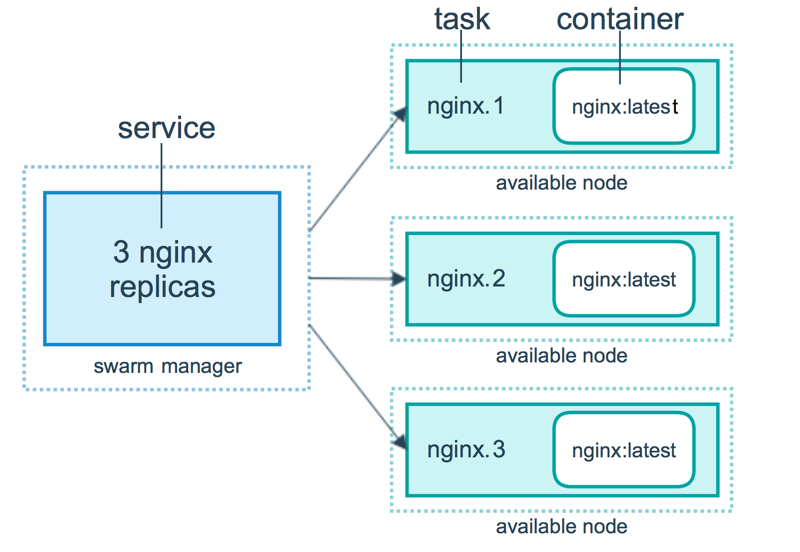
\includegraphics[scale=0.5]{figure/services-swarm.png}
\end{center}
\caption{Service deploy over a Swarm ~\label{services_swarm}}
\end{figure}
\\[1\baselineskip]
When a user deploys an application image in swarm mode, he is creating a \textbf{service}. Frequently a service is the image for a \textit{microservice} within the context of some larger application.\newline
In the service creation context, must be specified which container image to use and which commands to execute inside running containers, with the opportunity of defining:
\begin{itemize}
	\item the port where the swarm makes the service available outside the swarm
	\item an overlay network for the service to connect to other services in the swarm
	\item the number of replicas of the image to run in the swarm
\end{itemize}
When a service is deployed to the swarm, swarm manager accepts the service definition as the desired state for the service. Then it schedules the service on nodes in the swarm as one or more replica tasks. Tasks run independently of each other on nodes in the swarm \cite{DockerSwarm}.
\\[1\baselineskip]
In this project Docker is necessary in order to deploy Apache Spark and HDFS on a cluster of computers and so distribute the execution (horizontal scalability). In next chapters will be discussed how this service is deployed.

\section{Microsoft Azure}
Microsoft Azure is a Cloud Computing service created by Microsoft for building, testing, deploying, and managing applications and services through a global network of Microsoft-managed data centres. It provides Software as a Service (SaaS), Platform as a Service (PaaS) and Infrastructure as a Service (IaaS) and supports many different programming languages, tools and frameworks.\newline
\textbf{Cloud Computing} is a model for enabling convenient, on-demand network access to a shared pool of configurable computing resources (e.g., networks, servers, storage, applications, and services) that can be rapidly provisioned and released with minimal management effort or service provider interaction. Indeed with a power plant analogy, we can say it used to be that everyone had their own power source; then people started to build large, centralized power plants with very large capacity, connected to customers by a network. Their usage is metered, and everyone pays only for what they actually use.\newline
So using this approach, as shown in Figure \ref{static_cloud}, we can observe how the unused resources quantity, given as \[[Computational Capacity - Computational Demand]\]
decreases using the cloud, instead that provisioning a proper data centre.


\begin{figure}[h] 
\begin{center}
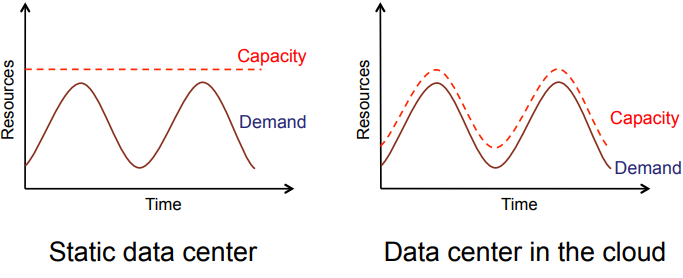
\includegraphics[scale=0.6]{figure/Static_data_center_Data_center_in_cloud.png}
\end{center}
\caption{Static data centre and Data centre in cloud ~\label{static_cloud}}
\end{figure}






